\documentclass[]{cv-style} % Add 'print' in [] to get print-view
\usepackage{graphicx}
\usepackage{xeCJK}
\usepackage{setspace}
\begin{document}
\header{ }{  }
\begin{aside}
\section{.}
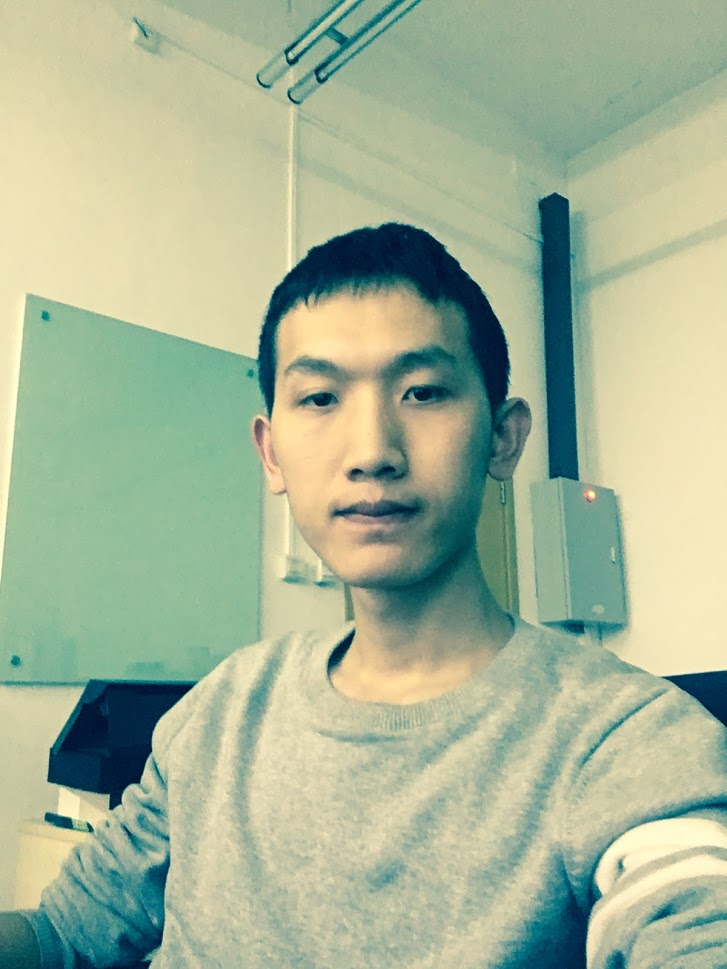
\includegraphics[width=4cm]{mathen}
\section{Contact}
网易游戏(杭州)
~
13581724604
~
hitminxuanwang\\@gmail.com
\section{Languages}
C++
Python
\section{Skills}
图形渲染OpenGL DX
图像处理OpenCV
\end{aside}
\section{Career Objective}
  \vspace{-0.2cm}
  \hspace{0.2cm}图形图像相关工作岗位,与图形图像相关的计算机视觉方向岗位,算法相关职位。
\section{Experience}
\begin{entrylist}

\entry
  {2018.7-Now}
  {图形学工程师}
  {网易游戏}
  {
    \vspace{-5pt}
    \leftmargini=-1cm
    \begin{itemize}
      \setlength{\itemsep}{3pt}
      \item {项目经验:GPU Instancing场景;实时软阴影;水彩风格化;卡通和PBR Shader; \\点光照明;软粒子特效;全屏后处理效果; 移动端优化;其他图形需求}
      \item {工程实现:Projective Texture; LiSPSM; Global Fog; Volumetric Fog; PBR}
      \item {理论学习: Real Time Rendering}
      \item {创新点:创建相机位置坐标系解决人物光照问题;Frustum分成3裁剪面固定Fov\\解决深度显示问题;}
    \end{itemize}
    \vspace{5pt}
    \hspace{-1.2cm} \textbf{keywords:} \emph{Rendering}, HLSL, OpenGL, 移动端优化, C++, Python
  }

\entry
  {2017.11-18.1}
  {实习生}
  {旷世科技}
  {
    \vspace{-5pt}
    \leftmargini=-1cm
    \begin{itemize}
      \setlength{\itemsep}{3pt}
      \item {提取人脸特征并快速检测Haar-like特征+积分图机制+级联分类器}
      \item {调研ImageCaption相关研究}
    \end{itemize}
    \vspace{5pt}
    \hspace{-1.2cm} \textbf{keywords:} \emph{Facial recognition, C++, LSTM}
  }

\entry
  {2017.6-7}
  {实习生}
  {网易游戏}
  {
    \vspace{-5pt}
    \leftmargini=-1cm
    \begin{itemize}
      \setlength{\itemsep}{3pt}
      \item {区别于传统计算方式,直接使用GPU生成光照贴图数据, 主要参考Unreal中的\\CPU的保守光栅, 移植到GPU端}
      \item {设置图像质量衡量指标筛选质量不达标的贴图}
    \end{itemize}
    \vspace{5pt}
    \hspace{-1.2cm} \textbf{keywords:} OpenGL, OpenCV, 图像处理, C++, Python
  }

\entry
  {2016 - 2017}
  {学生}
  {清华大学}
  {
    \vspace{-5pt}
    \leftmargini=-1cm
    \begin{itemize}
      \setlength{\itemsep}{3pt}
      \item {改进摄影构图的论文,根据用户拍摄的图像进行合适的构图推荐}
      \item {应用As Projective As Possible算法完成多图像对齐}
      \item {实现并比较多种图像融合算法:Multi-Splines,Modified Poisson,Convolution\\ Pyramid
      , Multi-Band,Mean-Value Coordinates等}
      \item {提出改进的卷积金字塔方法消除色彩渗透,生成效果更好的全景视频}
    \end{itemize}
    \vspace{5pt}
    \hspace{-1.2cm} \textbf{keywords:} \textbf{全景图像, 泊松方程, 调和插值, 频域卷积},{C++ , OpenCV}
}

\end{entrylist}
\vspace{-10pt}
\section{Education}
\begin{entrylist}
\vspace{-10pt}
\entry
{2015 - 2018}
{图形学与计算几何实验室 {\normalfont ~~ 计算机专业~~清华大学}}
{ 硕士}
{}
\vspace{-10pt}
\entry
{2010 - 2014}
{计算机专业 {\normalfont ~~ 哈尔滨工业大学}}
{ 学士}
{ }
\end{entrylist}
\vspace{-5pt} 
\section{Publications}
\begin{entrylist}
\entry
{2018}
{A Comparative Study of Algorithms for Realtime Panoramic Video Blending.}
{TIP}
{ IEEE Trans. Image Processing 27(6): 2952-2965 (2018)}
\entry
{2017}
{Avoiding bleeding in image blending.}
{ICIP}
{IEEE International Conference on Image Processing}
\end{entrylist}
\vspace{-10pt}
\section{Awards}
\begin{entrylist}
  \vspace{5pt}
   \hspace{0.2cm}研究生期间的全景视频生成项目获得清华-腾讯联合实验室优秀项目奖\\
   \hspace{0.2cm}全景视频生成项目作为实验室项目的一部分参与了国家科技进步二等奖的申报并获奖
\end{entrylist}

\end{document}